<<<<<<< HEAD
\documentclass{beamer}
\usepackage{media9}
\usepackage{subfig}
\title{The Sudoku Project}
\subtitle{Project Presentation}
\author[Ishika | Yashvi]{Ishika De and Yashvi Donga}
\date{24th October 2021}

\usetheme{Madrid}
\setbeamertemplate{navigation symbols}{}
\begin{document}
\begin{frame}
     \titlepage
\end{frame}
\begin{frame}
     \frametitle{Agenda}
     \begin{itemize}
          \item Overview
          \item Toolchain
          \item Brief Description
          \item Results
          \item Challenges
          \item Learnings
          \item Future Scope
     \end{itemize}
\end{frame}

\begin{frame}
     \frametitle{Overview}
     The goal of this project is to investigate a variety of algorithms (backtracking, brute force, stochastic search and Crook's algorithm) that are capable of solving sudoku puzzles, of ranging difficulties, in order to learn more about sudoku solving techniques.\newline

     We also wanted to use the OpenCV library to read a sudoku from an image and solve it.
\end{frame}

\begin{frame}
    \frametitle{Toolchain and Statistics}
    \begin{itemize}
         \item Languages: Python, C++ and Java
         \item Libaries used in Python: Numpy, OpenCV and Keras
         \item Total commits: 51
         \item Total lines of code: 2694
         %https://codetabs.com/count-loc/count-loc-online.html
    \end{itemize}
\end{frame}

\begin{frame}
     \frametitle{Brief Description}   
     \begin{itemize}
		  \item Tested backtracking and brute force algorithm
		     % \begin{figure}
               % \includegraphics[width=0.6\textwidth]{./backtrack.gif}
               % \caption{A representation of backtracking algorithm}
               % \end{figure}  
               \vspace{4mm}
               \begin{figure}
                    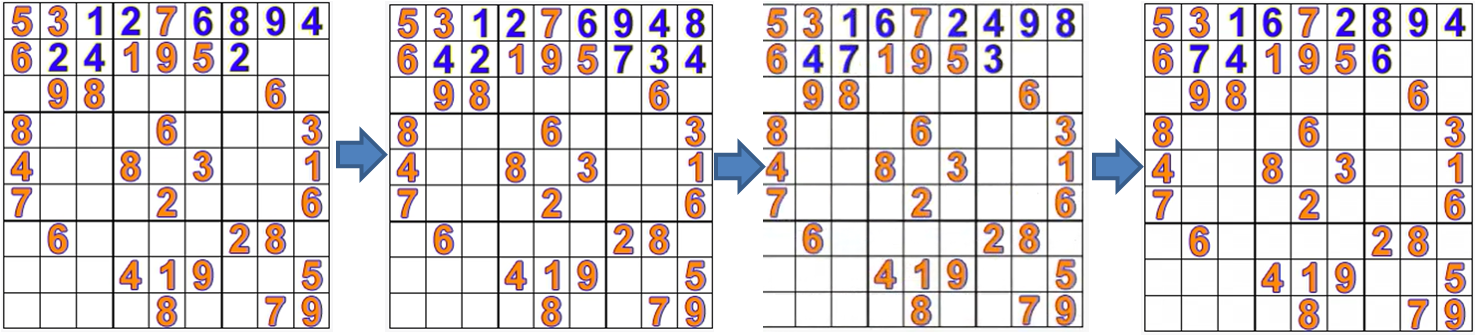
\includegraphics[width=0.6\textwidth]{./brute2.png}                  
                    \caption{A representation of backtracking algorithm}
                    \centering
                    \end{figure}   
               \begin{figure}                    
                    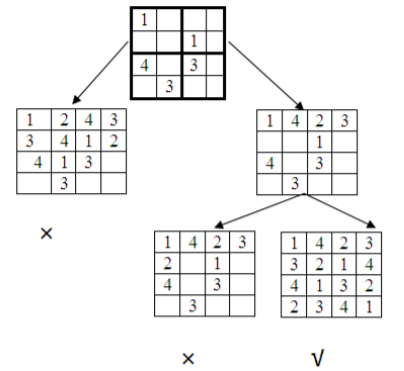
\includegraphics[width=0.3\textwidth]{./brute.png}
                    \caption{A representation of brute force algorithm}
                    \centering
                    \end{figure}        
	 \end{itemize}
\end{frame}

\begin{frame}
     \frametitle{Brief Description}   
     \begin{itemize}
          \item Tried implementing stochastic simulated annealing algorithm and Crook's algorithm
               \begin{figure}%
                    \centering
                    \subfloat[\centering Simulated annealing - Basics]{{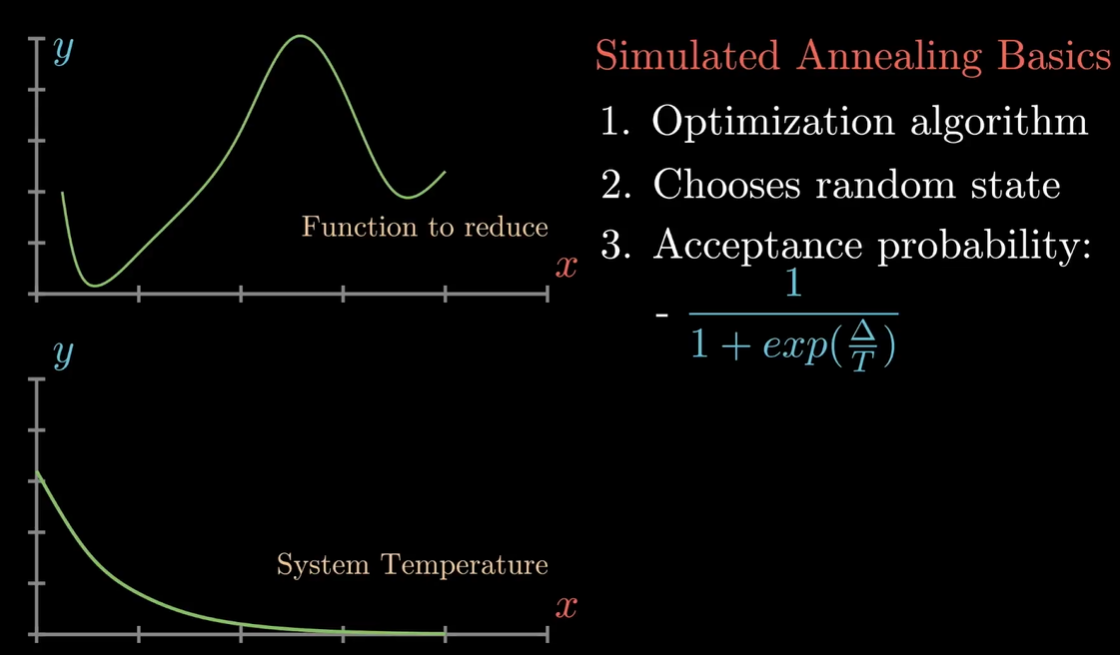
\includegraphics[width=5cm]{./siman.png} }}%
                    \qquad
                    \subfloat[\centering Representation of Crook's algorithm]{{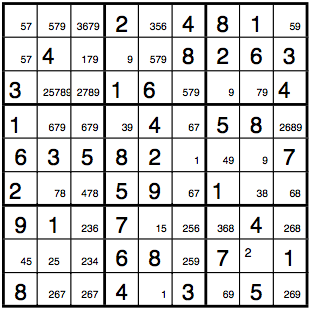
\includegraphics[width=3cm]{./crook.png} }}%
                    \label{fig:example}%
                \end{figure}
	 \end{itemize}
\end{frame}

\begin{frame}
     \frametitle{Brief Description}   
     \begin{itemize}
		  \item Generated random sudoku puzzles
		  \item Recognized a sudoku from an image and solved it
		  \begin{figure}
               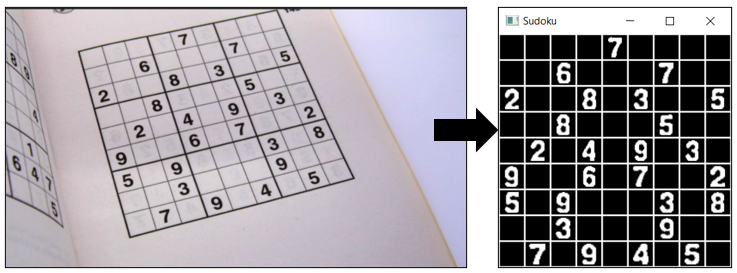
\includegraphics[width=0.8\textwidth]{./week9_img/transformation.png}
               \caption{Image after processing}
               \end{figure}
	 \end{itemize}
\end{frame}

\begin{frame}
     \frametitle{Results}   
		  \begin{figure}
		  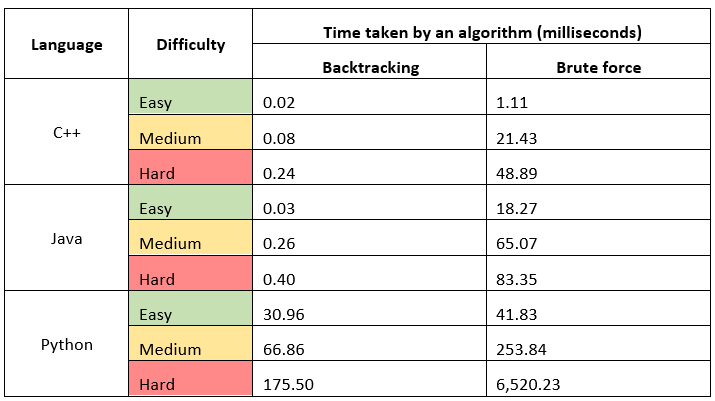
\includegraphics[width=0.9\textwidth]{./week9_img/data.png}
		  \caption{Average time taken to solve a sudoku (tested 100 puzzles).}
		  \centering
		  \end{figure}
\end{frame}

\begin{frame}
    \frametitle{Challenges}   
    \begin{itemize}
         \item Setting unrealistic deadlines
         \item Explaining each other’s ideas/concepts
         \item Failure to implement a few algorithms
         \item Dealing with code errors
    \end{itemize}
\end{frame}

\begin{frame}
     \frametitle{Learnings}
     \begin{itemize}
		 \item Collaborate using git 
		 \item Write the same algorithm in different languages
		 \item Explain our code, thought processess and ideas to each other
		 \item Apply the concept of cost function and thermodynamics in simulated annealing
		 \item Process an image to extract digits of a sudoku
		 \item Implement neural networks to predict digits of a sudoku from an image
		 \item Importance of changeability of code
	 \end{itemize}
\end{frame}

\begin{frame}
    \frametitle{Future Scope}   
    \begin{itemize}
         \item Implement a sudoku solver in Haskell and Elixir
         \item Explore more algorithms like dancing links algorithm
    \end{itemize}
\end{frame}

\begin{frame}
    \centering \huge \huge {Thank You}
\end{frame}

\end{document}




=======
\documentclass{beamer}
\title{The Sudoku Project}
\subtitle{Project Presentation}
\author[Ishika | Yashvi]{Ishika De and Yashvi Donga}
\date{24th October 2021}

\usetheme{Madrid}

\begin{document}
\begin{frame}
     \titlepage
\end{frame}
\begin{frame}
     \frametitle{Agenda}
     \begin{itemize}
          \item Overview
          \item Toolchain
          \item Brief Description
          \item Challenges
          \item Learnings
          \item Future Scope
     \end{itemize}
\end{frame}

\begin{frame}
     \frametitle{Overview}
     The goal of this project is to investigate a variety of algorithms (backtracking, brute force, stochastic search and Crook's algorithm) that are capable of solving sudoku puzzles, of ranging difficulties, in order to learn more about sudoku solving techniques.\newline

     We also wanted to use the OpenCV library to read a sudoku from an image and solve it.
\end{frame}

\begin{frame}
    \frametitle{Toolchain}
    \begin{itemize}
         \item Languages: Python, C++ and Java
         \item Libaries used in Python: Numpy, OpenCV and Keras
    \end{itemize}
\end{frame}

\begin{frame}
     \frametitle{Brief Description}   
     \begin{itemize}
		  \item Tested backtracking and brute force algorithm
		  \item Tried implementing stochastic simulated annealing algorithm and Crook's algorithm
		  \item Generated random sudoku puzzles
		  \item Recognized a sudoku from an image and solved it
	 \end{itemize}
\end{frame}

\begin{frame}
     \frametitle{Results}   
		  \begin{figure}
		  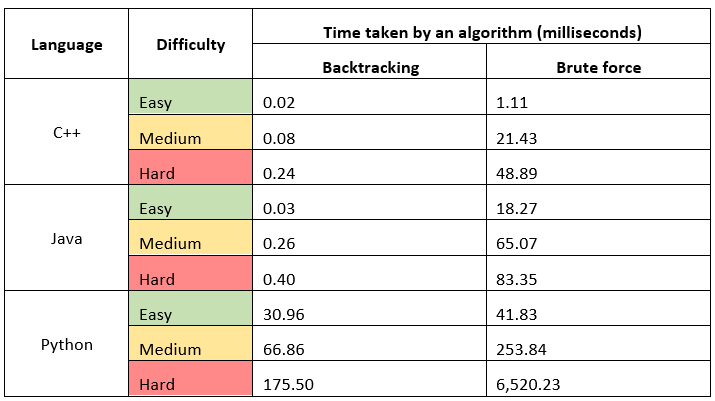
\includegraphics[width=0.9\textwidth]{./week9_img/data.png}
		  \caption{Average time taken to solve a sudoku (tested 100 puzzles).}
		  \centering
		  \end{figure}
\end{frame}

\begin{frame}
	\frametitle{Results}
		  \begin{figure}
		  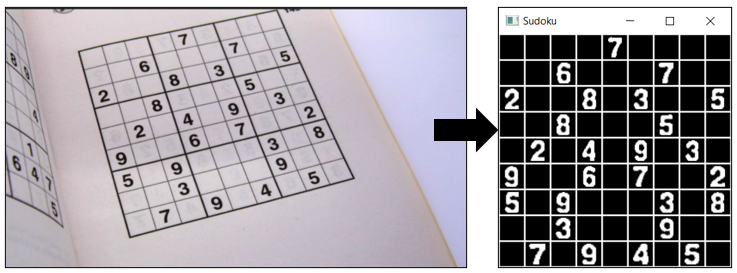
\includegraphics[width=0.6\textwidth]{./week9_img/transformation.png}
		  \caption{Image processing of a sudoku.}
		  \centering
		  \end{figure}

          \begin{figure}
            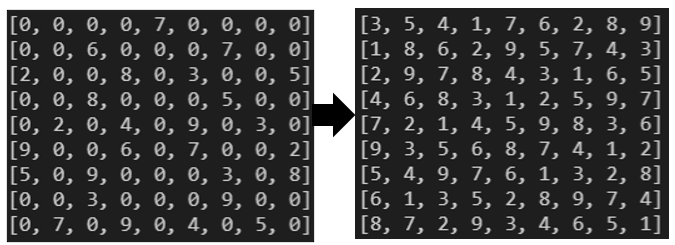
\includegraphics[width=0.6\textwidth]{./week9_img/solve.PNG}
          \caption{Solved the sudoku from the image}
          \centering
        \end{figure}
\end{frame}

\begin{frame}
    \frametitle{Challenges}   
    \begin{itemize}
         \item Setting unrealistic deadlines
         \item Explaining each other’s ideas/concepts
         \item Failure to implement a few algorithms
         \item Dealing with code errors
    \end{itemize}
\end{frame}

\begin{frame}
     \frametitle{Learnings}
     \begin{itemize}
		 \item Collaborate using git
		 \item Write the same algorithm in different languages
		 \item Explain our code, thought processess and ideas to each other
		 \item Apply the concept of cost function and thermodynamics in simulated annealing
		 \item Process an image to extract digits of a sudoku
		 \item Implement neural networks to predict digits of a sudoku from an image
		 \item Importance of changeability of code
	 \end{itemize}
\end{frame}

\begin{frame}
    \frametitle{Future Scope}   
    \begin{itemize}
         \item Implement a sudoku solver in Haskell and Elixir
    \end{itemize}
\end{frame}

\begin{frame}
    \centering \huge {Thank You}
\end{frame}

\end{document}




>>>>>>> 6431899b638243e16e5dd69d4ee6edcaf7c26bce
